\chapter{Performance and Fault Tolerance}
\label{ch:performance}

Tendermint is designed as a Byzantine fault tolerant state-machine replication algorithm.
It guarantees safety so long as less than a third of validators are Byzantine, 
and guarantees liveness similarly, so long as network messages are eventually delivered,
with weak assumptions about network synchrony for gossiping proposals.
In this section, we evaluate Tendermint's fault tolerance empirically by injecting 
crash faults and Byzantine faults.
The goal is to show that the implementation of Tendermint consensus does not compromise safety in the event of such failures,
that it suffers minimum performance impact, and that it is quick to recover.

Performance of the Tendermint algorithm can be evaluated in a few key ways.
The most obvious measures are the block commit time, which is a measure of finalization latency, 
and transaction throughput, which measures the network's capacity.
We collect measurements for each on networks with validators distributed over the globe, 
where the number of validators ranges, in multiples of 2, from 2 to 64.

\section{Overview}

The experiments in this chapter can be reproduced using the repository at \url{https://github.com/tendermint/network\_testing}.
All experiments except one take place in docker containers 
running on \emph{Amazon EC2} instances of type \emph{t2.medium}.
The \emph{t2.medium} has 2 vCPU and 4 GB of RAM.
One experiment tests the throughput on larger instances, the \emph{c3.8xlarge}, 
which has 32 vCPUs and 60 GB of RAM.
Instances are distributed across seven datacenters, spanning five continents.
A second docker container, responsible for generating transactions, is run on each instance.
Transactions are 250 bytes in size (a reasonable size for including a few 32 or 64 byte hashes and signatures),
and were constructed to be debuggable, to be quick to generate, and to contain some stochasticity.
Thus, the leading bytes are Big-Endian encoded integers 
representing transaction number and validator index for that instance,
the trailing 16 bytes are randomly drawn from the operating system, 
and the intermediate bytes are just zeros.

A network monitoring tool is used to maintain active websocket connections 
to each validator's Tendermint RPC server,
and uses its local time when it receives a new committed block 
for the first time as the official commit time for that block.
Experiments were first run without the monitor by copying 
all data from the validators for analysis and using the local time
of the 2/3th validator committing a block as the commit time. 
Using the monitor is much faster, amenable to online monitoring, 
and was found to not impact the results 
so long as only block header information (and not the whole block) was passed over the websockets.

Docker containers on remote machines are easily managed using the \emph{docker-machine} tool, 
and the network\_testing repository provides some tools 
which take advantage of Go's concurrency features
to perform actions on docker containers on many remote machines at once.

Each validator connects directly to each other to avoid confounding effects of network topology.

For experiments involving crash faults or Byzantine behaviour, 
the number of faulty nodes is given by $N_{fault} = \lfloor(N-1)/3\rfloor$,
where $N$ is the total number of validators.

\section{Throughput and Latency}

This section describes experiments which measure the raw performance 
of Tendermint in non-adversarial conditions,
where all nodes are online and synced and no accommodations are made for asynchrony.
That is, an artificially high TimeoutPropose is used (10 seconds), 
and all other timeout parameters are set to 1 millisecond.
Additionally, all mempool activity is disabled 
(no gossiping of transactions or rechecking them after commits),
and an in-process nil application is used to bypass TMSP.
This serves as a control scenario for evaluating the performance drop in the face of faults and/or asynchrony.

Experiments are run on validator set sizes doubling in size from two to 64, and on block sizes doubling from 128 to 32768.
Transactions are preloaded on each validator. Each experiment is run for 16 blocks. 

\begin{figure}[]
	\centering
	\begin{subfigure}{0.8 \textwidth}
		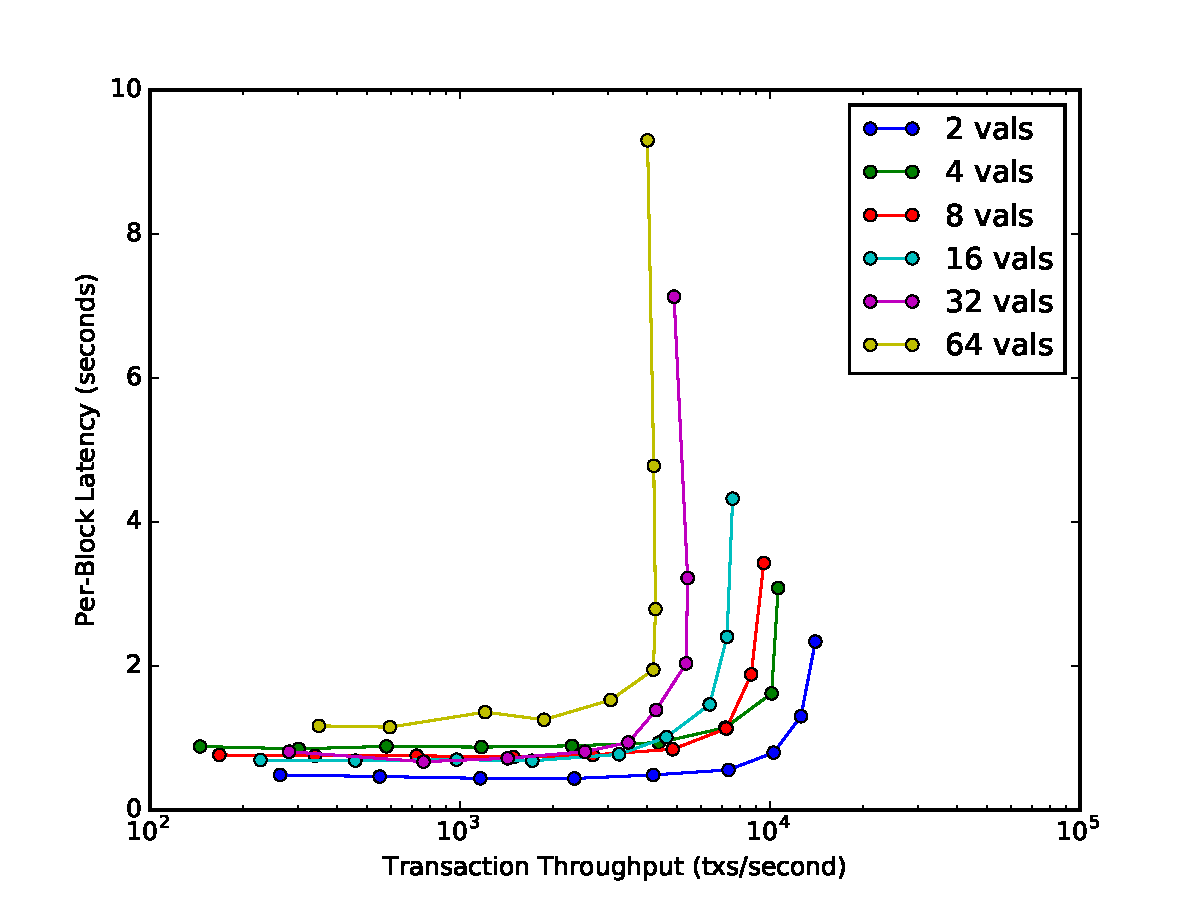
\includegraphics[width=\linewidth,height=\textheight,keepaspectratio]{figures/throughput/latency-throughput.pdf}
	\end{subfigure}

	\begin{subfigure}{0.8 \textwidth}
		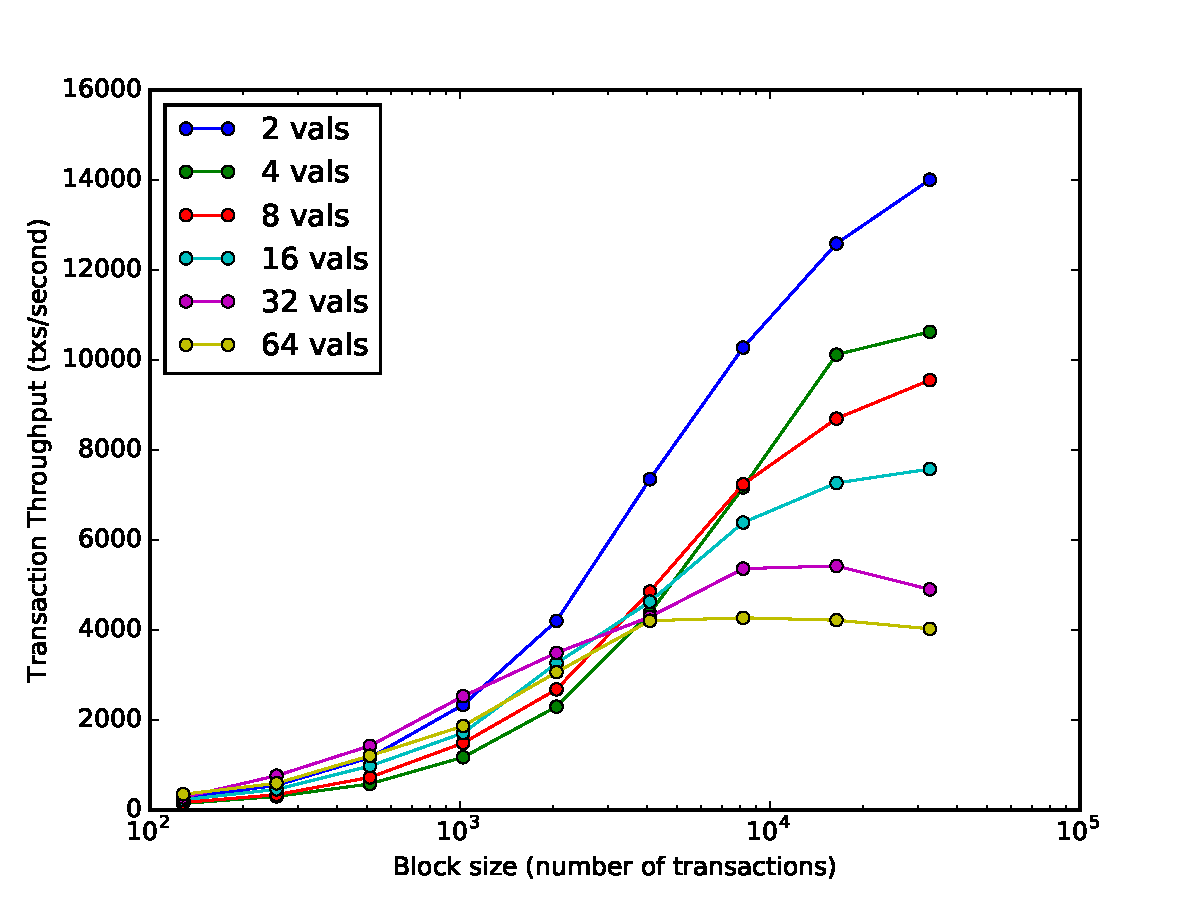
\includegraphics[width=\linewidth,height=\textheight,keepaspectratio]{figures/throughput/throughput-blocksize.pdf}
	\end{subfigure}
	\centering
	\caption[Latency-Throughput trade-off in non-faulty global network]{Latency-throughput trade-off.
Larger blocks incur diminishing 
returns in transaction throughput, with an ultimate capacity at around 10,000 txs/s}
	\label{fig:exp:throughput}
\end{figure}

As can be seen in Figure \ref{fig:exp:throughput},
Tendermint easily handles thousands of transactions per second with around one second block latency,
though there appears to be a capacity limit at around ten thousand transactions per second.
A block of 16384 transactions is about 4 MB in size, and analysis of network bandwidth shows each connection
easily reaching upwards of 20MB/s, though analysis of the logs shows that at high block sizes, 
validators can spend upwards of two seconds waiting for block parts.
Additionally, experiments in single data centers, as shown in Figure \ref{fig:exp:throughput:single},
demonstrate that much higher throughputs are possible,
while experiments on much larger machines exhibit more consistent performance,
relieving the capacity limit, as shown in Figure \ref{fig:exp:throughput:large}.
We leave further investigations of this capacity limit to future work.

\begin{figure}[]
	\centering
	\begin{subfigure}{0.8 \textwidth}
		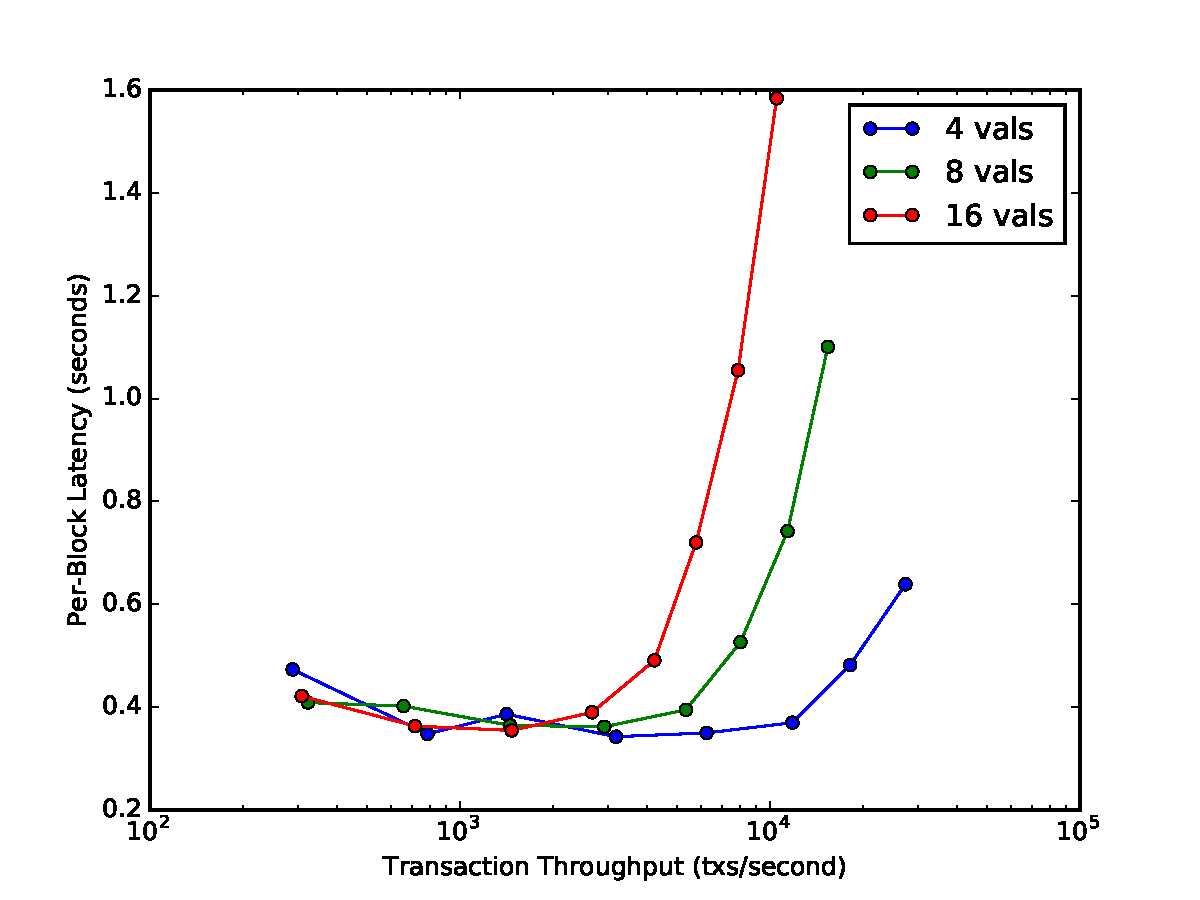
\includegraphics[width=\linewidth,height=\textheight,keepaspectratio]{figures/throughput/single_datacenter/latency-throughput.pdf}
		\centering
	\end{subfigure}

	\begin{subfigure}{0.8 \textwidth}
		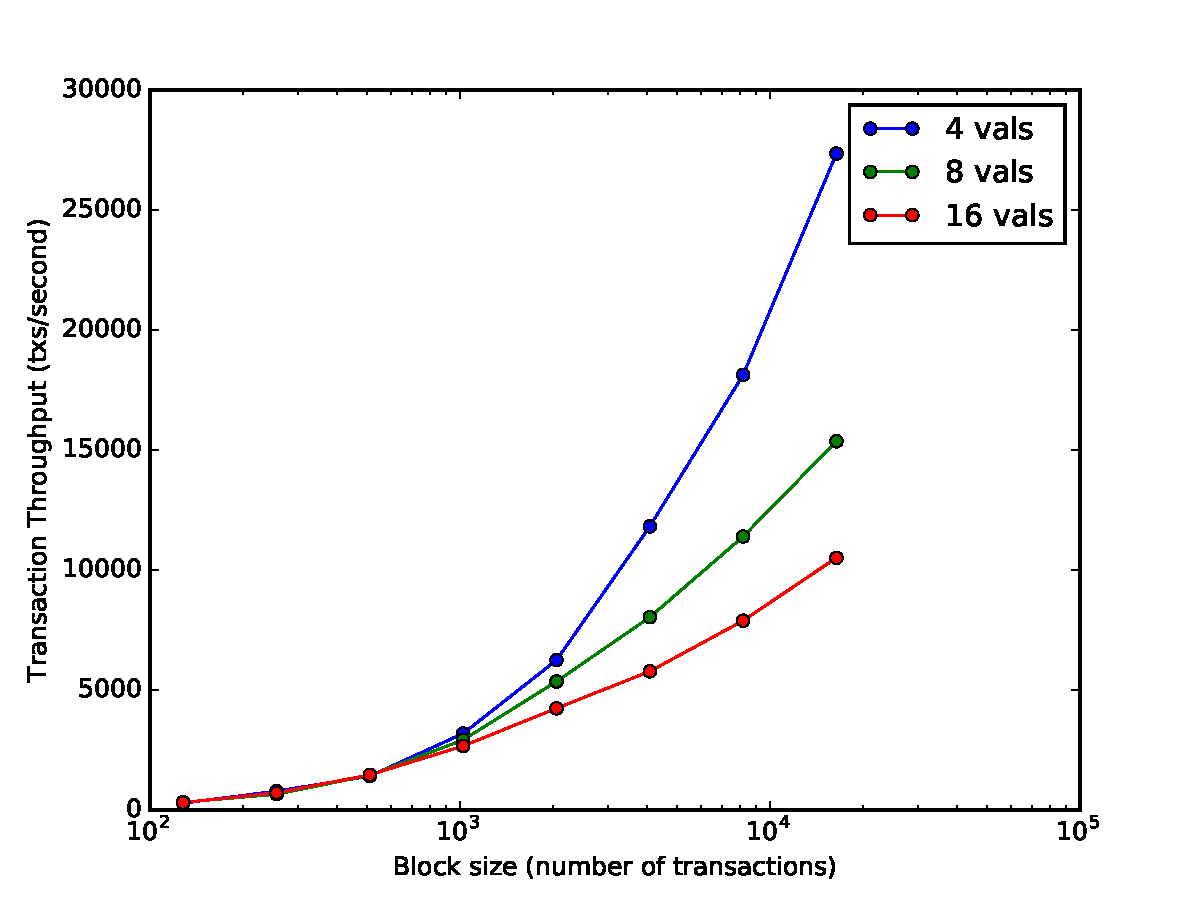
\includegraphics[width=\linewidth,height=\textheight,keepaspectratio]{figures/throughput/single_datacenter/throughput-blocksize.pdf}
	\end{subfigure}
	\caption[Latency-throughput trade-off in non-faulty local network]{Single datacenter.
When messages don't need to cross the public Internet, Tendermint is capable of tens of thousands of transactions per second.}
	\label{fig:exp:throughput:single}
\end{figure}



\begin{figure}[]
	\centering
	\begin{subfigure}{0.8 \textwidth}
		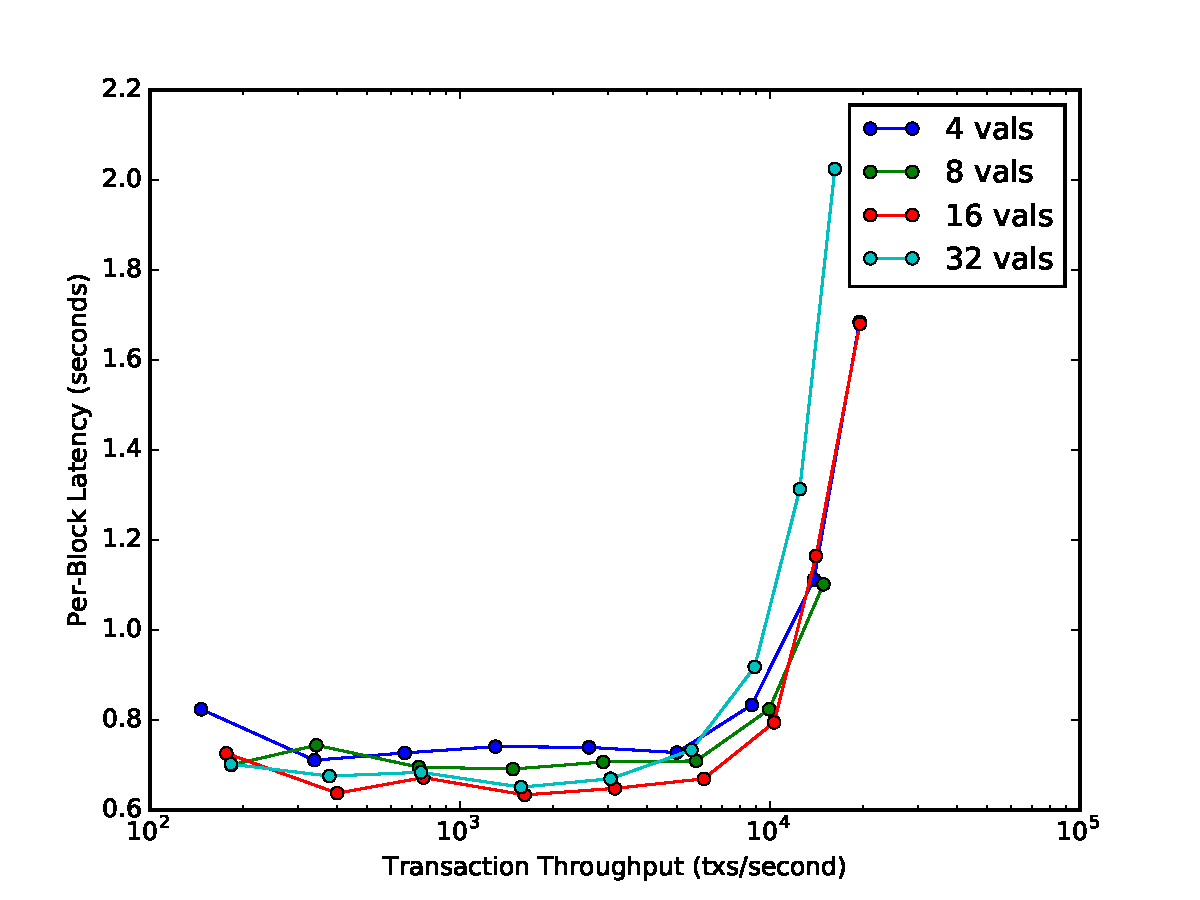
\includegraphics[width=\linewidth,height=\textheight,keepaspectratio]{figures/throughput/large_instances/latency-throughput.pdf}
		\centering
	\end{subfigure}

	\begin{subfigure}{0.8 \textwidth}
		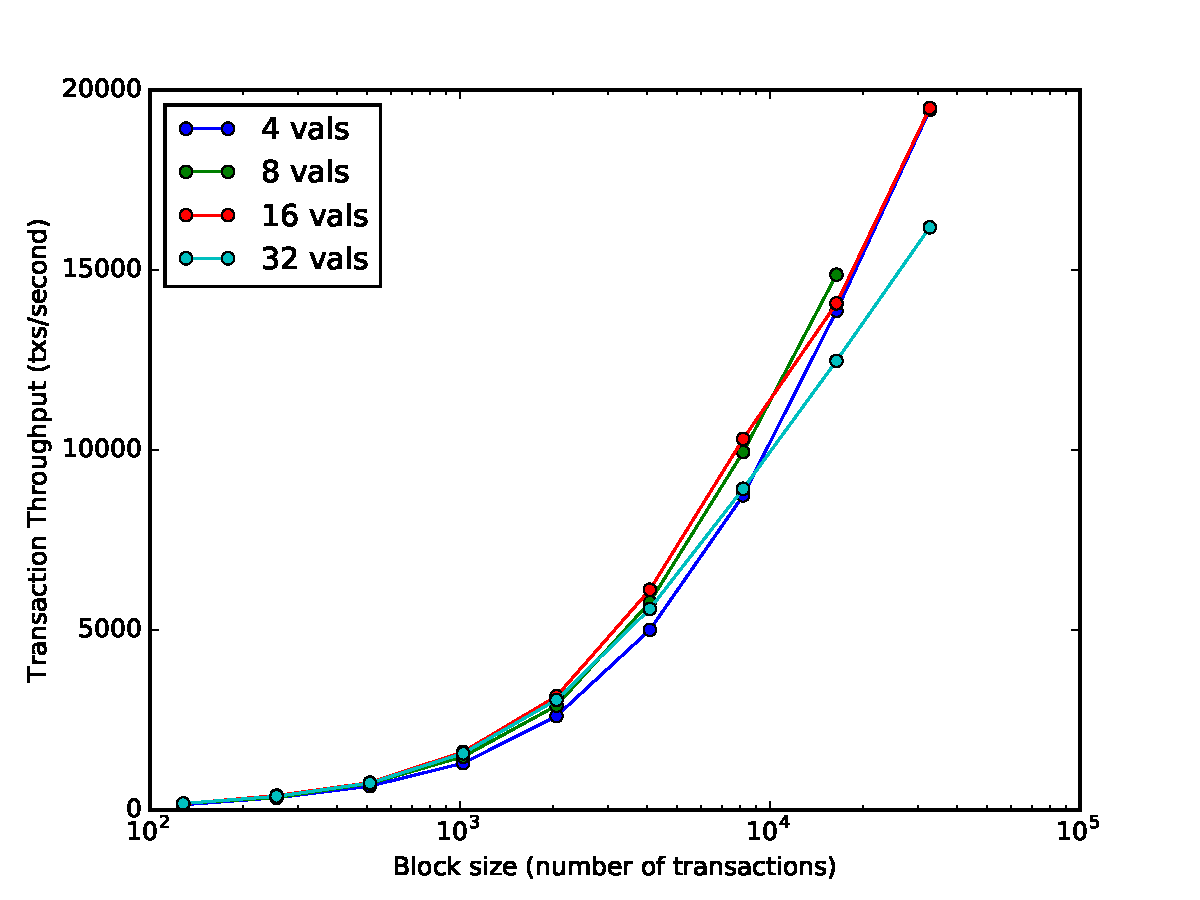
\includegraphics[width=\linewidth,height=\textheight,keepaspectratio]{figures/throughput/large_instances/throughput-blocksize.pdf}
	\end{subfigure}
	\centering
	\caption[Latency-Throughput trade-off in non-faulty global network of large machines]{Large machines.
With 32 vCPU and 60 GB of RAM, transaction throughput increases linearly with block-size, 
relieving the capacity limits found on smaller machines.}
	\label{fig:exp:throughput:large}
\end{figure}

In the experiments that follow, various forms of fault are injected
and latency statistics presented.
Each experiments was run for validator set sizes doubling from 4 to 32, 
for varying values of TimeoutPropose, and with a block size of 2048 transactions.

\section{Crash Failures}

To evaluate the performance of a network subject to crash failures, 
every three seconds $N_{fault}$ validators were randomly selected,
stopped, and restarted three seconds later.

The results in Table \ref{fig:exp:crash_failure} demonstrate that 
performance under this crash failure scenario drops by about 
$50\%$, and that larger TimeoutPropose values help mediate latencies. 
While the average latency increases to about two seconds,
the median is closer to one second, and latencies may run as high as ten or twenty seconds,
though in one case it was as high as seventy seconds.
It is likely that modifying TimeoutPropose to be slightly non-deterministic may
ease the probability of such extreme latencies.

\begin{table}
	4 Validators

\begin{center}
	\begin{tabular}{| l | l | l | l | l | l | }
		\hline
		TimeoutPropose & Min & Max & Mean & Median & $95^{th} \ \%-ile$ \\ \hline
		500 & 434 & 15318 & 2179 & 1102 & 5575 \\ \hline
		1000 & 516 & 18149 & 2180 & 1046 & 5677 \\ \hline
		2000 & 473 & 15067 & 2044 & 1049 & 5479 \\ \hline
		3000 & 428 & 9964 & 2005 & 1096 & 5502 \\ \hline
	\end{tabular}
\end{center}

8 Validators

\begin{center}
	\begin{tabular}{| l | l | l | l | l | l | }
		\hline
		TimeoutPropose & Min & Max & Mean & Median & $95^{th} \ \%-ile$ \\ \hline
		500 & 618 & 126481 & 2679 & 990 & 5589 \\ \hline
		1000 & 570 & 9832 & 1763 & 962 & 5835 \\ \hline
		2000 & 594 & 8869 & 1658 & 968 & 5481 \\ \hline
		3000 & 535 & 10101 & 1633 & 959 & 5485 \\ \hline
	\end{tabular}
\end{center}

16 Validators

\begin{center}
	\begin{tabular}{| l | l | l | l | l | l | }
		\hline
		TimeoutPropose & Min & Max & Mean & Median & $95^{th} \ \%-ile$ \\ \hline
		500 & 782 & 21354 & 1977 & 1001 & 5930 \\ \hline
		1000 & 758 & 12659 & 1761 & 981 & 5642 \\ \hline
		2000 & 751 & 21285 & 2041 & 1005 & 6872 \\ \hline
		3000 & 719 & 72406 & 2395 & 991 & 5987 \\ \hline
	\end{tabular}
\end{center}

32 Validators

\begin{center}
	\begin{tabular}{| l | l | l | l | l | l | }
		\hline
		TimeoutPropose & Min & Max & Mean & Median & $95^{th} \ \%-ile$ \\ \hline
		500 & 760 & 24692 & 2591 & 1087 & 14025 \\ \hline
		1000 & 755 & 19696 & 2328 & 1119 & 9321 \\ \hline
		2000 & 852 & 21044 & 2178 & 1141 & 6514 \\ \hline
		3000 & 763 & 25587 & 2289 & 1119 & 6707 \\ \hline
	\end{tabular}
\end{center}


	\caption[Latency statistics under crash faults]{Crash-fault latency statistics. Every three seconds, a random selection of$N_{fault}$ validators were crashed, and restarted three seconds later. This crash-restart procedure continued for 200 blocks. Each table reports the minimum, maximum, average, median, and $95^{th}$ percentile of the block latencies, for varying values of the TimeoutPropose parameter.}
	\label{fig:exp:crash_failure}
\end{table}

\section{Random Network Delay}

Another form of fault, which may attributed either to Byzantine behaviour or to network asynchrony,
is to inject random delays into every read and write to a network connection.
In this experiment, before every read and write on every network connection,
$N_{fault}$ of the validators slept for $X$ milliseconds, 
where $X$ was drawn uniformly on $(0, 3000)$.
As can be seen in Table \ref{fig:exp:delay}, 
latencies are similar to the crash failure scenario, 
though increasing the TimeoutPropose has the opposite effect.
Since not all validators were faulty, 
small values of TimeoutPropose allow faulty validators to be skipped quickly. 
If all validators were subject to the network delays, 
larger TimeoutPropose values would be expected to reduce latency
since there would be no non-faulty validators to skip to,
and more time would be provided to received delayed messages.

\begin{table}[]
	
\begin{subtable}{.5 \linewidth}
	\centering
	\begin{tabular}{| l | l | l | l | l | l | }
		\hline
		TimeoutPropose & Min & Max & Mean & Median & $95^{th} \ \%-ile$ \\ \hline
		1000 & 873 & 2796 & 1437 & 1036 & 2627 \\ \hline
		2000 & 831 & 4549 & 1843 & 1180 & 4036 \\ \hline
		3000 & 921 & 5782 & 2273 & 1251 & 5491 \\ \hline
		4000 & 967 & 6875 & 2700 & 1413 & 6781 \\ \hline
	\end{tabular}
	\caption{4 Validators}
\end{subtable}


\begin{subtable}{.5 \linewidth}
	\centering
	\begin{tabular}{| l | l | l | l | l | l | }
		\hline
		TimeoutPropose & Min & Max & Mean & Median & $95^{th} \ \%-ile$ \\ \hline
		1000 & 870 & 2840 & 1449 & 1040 & 2786 \\ \hline
		2000 & 957 & 4268 & 1848 & 1076 & 4148 \\ \hline
		3000 & 859 & 5724 & 2156 & 1100 & 5649 \\ \hline
		4000 & 897 & 11859 & 3055 & 1093 & 11805 \\ \hline
	\end{tabular}
	\caption{8 Validators}
\end{subtable}


\begin{subtable}{.5 \linewidth}
	\centering
	\begin{tabular}{| l | l | l | l | l | l | }
		\hline
		TimeoutPropose & Min & Max & Mean & Median & $95^{th} \ \%-ile$ \\ \hline
		1000 & 914 & 5595 & 1821 & 1135 & 5466 \\ \hline
		2000 & 950 & 7782 & 2490 & 1165 & 7650 \\ \hline
		3000 & 978 & 10305 & 3049 & 1163 & 9890 \\ \hline
		4000 & 1018 & 6890 & 2808 & 1174 & 6813 \\ \hline
	\end{tabular}
	\caption{16 Validators}
\end{subtable}


\begin{subtable}{.5 \linewidth}
	\centering
	\begin{tabular}{| l | l | l | l | l | l | }
		\hline
		TimeoutPropose & Min & Max & Mean & Median & $95^{th} \ \%-ile$ \\ \hline
		1000 & 1202 & 8562 & 2219 & 1349 & 5733 \\ \hline
		2000 & 1196 & 7878 & 2549 & 1365 & 7579 \\ \hline
		3000 & 1164 & 10082 & 3003 & 1382 & 9805 \\ \hline
		4000 & 1223 & 17571 & 3696 & 1392 & 12014 \\ \hline
	\end{tabular}
	\caption{32 Validators}
\end{subtable}


	\caption[Latency statistics under randomized delays]{Random delay latency statistics. $N_{fault}$ validators were set to inject a random delay
before every read and write, where the delay time was chosen uniformly on $(0, 3000)$ milliseconds.}
	\label{fig:exp:delay}
\end{table}


\section{Byzantine Failures}

A more explicit Byzantine failure can be injected through the following modifications
to the state machine:

\begin{itemize}
\item{Conflicting proposals: during its time to propose, a Byzantine validator signs two conflicting proposals and broadcasts each, along with a pre-vote and pre-commit, to separate halves of its connected peers.} 
\item{No nil votes: a Byzantine validator never signs a nil-vote.}
\item{Sign every proposal: a Byzantine validator submits a pre-vote and a pre-commit for every proposal it sees, as soon as it sees it.}
\end{itemize}

Taken together, these behaviours explicitly violate the double signing and locking rules. 
Note, however, that the behaviour is dominated by the broadcast of conflicting proposals,
and the eventual committing of one of them.
More complex arrangements of Byzantine strategies are left for future work.
 
Despite the injected Byzantine faults, 
which would cause many systems to fail completely and immediately,
Tendermint maintains respectable latencies, as can be seen from Table \ref{fig:exp:byz_failure}.
Since these faults have little to do with asynchrony,
there is no real discernible effect from TimeoutPropose.
The performance also falls off with larger validator sets,
which may be the result of a naive algorithm for handling Byzantine votes.

\begin{table}[]
	
\begin{subtable}{.5 \linewidth}
	\centering
	\begin{tabular}{| l | l | l | l | l | l | }
		\hline
		TimeoutPropose & Min & Max & Mean & Median & $95^{th} \ \%-ile$ \\ \hline
		1000 & 868 & 3888 & 1450 & 1086 & 3320 \\ \hline
		2000 & 929 & 4375 & 1786 & 1272 & 4166 \\ \hline
		3000 & 881 & 4363 & 1224 & 1099 & 1680 \\ \hline
		4000 & 824 & 8256 & 1693 & 1272 & 2607 \\ \hline
	\end{tabular}
	\caption{4 Validators}
\end{subtable}


\begin{subtable}{.5 \linewidth}
	\centering
	\begin{tabular}{| l | l | l | l | l | l | }
		\hline
		TimeoutPropose & Min & Max & Mean & Median & $95^{th} \ \%-ile$ \\ \hline
		1000 & 771 & 3445 & 1472 & 916 & 3288 \\ \hline
		2000 & 731 & 3661 & 1426 & 902 & 3339 \\ \hline
		3000 & 835 & 6402 & 1912 & 962 & 6155 \\ \hline
		4000 & 811 & 4462 & 1512 & 964 & 3592 \\ \hline
	\end{tabular}
	\caption{8 Validators}
\end{subtable}


\begin{subtable}{.5 \linewidth}
	\centering
	\begin{tabular}{| l | l | l | l | l | l | }
		\hline
		TimeoutPropose & Min & Max & Mean & Median & $95^{th} \ \%-ile$ \\ \hline
		1000 & 877 & 15930 & 2086 & 1024 & 5844 \\ \hline
		2000 & 808 & 5737 & 1580 & 1027 & 4155 \\ \hline
		3000 & 919 & 10533 & 1801 & 1110 & 4174 \\ \hline
		4000 & 915 & 5589 & 1745 & 1095 & 4181 \\ \hline
	\end{tabular}
	\caption{16 Validators}
\end{subtable}


\begin{subtable}{.5 \linewidth}
	\centering
	\begin{tabular}{| l | l | l | l | l | l | }
		\hline
		TimeoutPropose & Min & Max & Mean & Median & $95^{th} \ \%-ile$ \\ \hline
		1000 & 1594 & 11730 & 2680 & 1854 & 5016 \\ \hline
		2000 & 1496 & 17801 & 3430 & 1874 & 11730 \\ \hline
		3000 & 1504 & 15963 & 3280 & 1736 & 9569 \\ \hline
		4000 & 1490 & 24836 & 3940 & 1773 & 12866 \\ \hline
	\end{tabular}
	\caption{32 Validators}
\end{subtable}


	\caption[Latency statistics under Byzantine faults]{Byzantine-fault latency statistics.
Byzantine validators propose conflicting blocks and vote on any proposal as soon as they see it.
Each table reports the minimum, maximum, average, median, and $95^{th}$ percentile of the block latencies, for varying values of the TimeoutPropose parameter.}
	\label{fig:exp:byz_failure}
\end{table}

\ifx
\section{A real application: ErisDB}

The experiments presented so far have been artificial to the extent that transactions incur no processing logic.
This was done deliberately to benchmark the core consensus engine. 
To get a handle on a real application, we present throughput and latency results for ErisDB, 
a blockchain application developed primarily by the author at Eris Industries, in collaboration with Jae Kwon.
ErisDB provides a rich set of features, including a native currency, the Ethereum Virtual Machine (EVM).
a native name registry, and a rich permissioning system.
Transactions must be digitally signed using ED25519 signatures to be valid, and all state queries and updates are done on a merkle IAVL tree.

For this experiment, a simple contract with two methods, get and set, is deployed to the virtual machine.
The contract is written in solidity, a high-level, javascript-like language developed by Ethereum which compiles down to EVM byte code.
The application state is preloaded with 1000 accounts, and transactions are signed by private keys drawn uniformly from those accounts.
Keys and values for the get and set methods are fixed at 32-bytes each, to reflect the native architecture of the EVM \cite{ethereum_yellow_paper}.
Transactions are generated for a read/write load of 10/90 (i.e. 90\% of transaction call the set method).

\fi

\section{Related Work}

The throughput experiments in this chapter were modeled after those in \cite{honeybadger},
which benchmarks the performance of a PBFT implementation 
and a new randomized BFT protocol called HoneyBadgerBFT.
In their results, PBFT achieves over 15,000 transactions per second on four nodes,
but decays exponentially as the number of nodes increases, 
while HoneyBadgerBFT attains roughly even performance
of between 10,000 and 15,000 transactions per second.
Block latencies in HoneyBadgerBFT, however, are much higher, 
closer to 10 seconds for validator sets of size 8, 16, and 32, and even more for larger ones.

A well known tool for studying consensus implementations is Jepsen \cite{jepsen},
which is used to test the consistency guarantees of databases by simulating 
many forms of network partition. 
Testing Tendermint with Jepsen remains an exciting area for future work.

The author is not aware of any throughput experiments in the face of persistent Byzantine failures,
like those presented here.

\section{Conclusion}

The implementation of Tendermint written by the author and Jae Kwon easily achieves 
thousands of transactions per second on up to 64 nodes on machines distributed around the globe, 
with latencies mostly in the one to two second range.
This is highly competitive with other solutions, and especially with the current state of blockchains,
with Bitcoin, for instance, capping out at around 7 transactions per second.
Furthermore, our implementation is shown to be robust to both crash faults, message delays,
and deliberate Byzantine faults,
being able to maintain over a thousand transactions per second in each scenario.


